% !TEX TS-program = xelatex
% !TEX spellcheck = en-US

%%%%%%%%%%%%%%%%%%%%%%%%%%%%%%%%%%%%%%%%%
% Twenty Seconds Resume/CV
% LaTeX Template
% Version 1.0 (14/7/16)
%
% Original author:
% Carmine Spagnuolo (cspagnuolo@unisa.it) with major modifications by
% Vel (vel@LaTeXTemplates.com) and Harsh (harsh.gadgil@gmail.com)
%
% License:
% The MIT License (see included LICENSE file)
%
%%%%%%%%%%%%%%%%%%%%%%%%%%%%%%%%%%%%%%%%%

% XeLaTex

%----------------------------------------------------------------------------------------
%  PACKAGES AND OTHER DOCUMENT CONFIGURATIONS
%----------------------------------------------------------------------------------------

\documentclass[a4paper]{twentysecondcv} % a4paper for A4

\usepackage{hyperref}
% DO EDIT THIS FILE DIRECTLY!
% This file is generated from data in YAML file ../../../_data/cv.yaml via 'make cv_update_tex'

\hypersetup{
pdftitle={John Paul Newman CV},
pdfsubject={CV},
pdfauthor={John Paul Newman},
pdfkeywords={CV}
}


%%% Configure a directory location for sections
\newcommand*{\sectiondir}{sections/}

% Command for printing skill overview
\newcommand\skills{
\vspace{4mm}
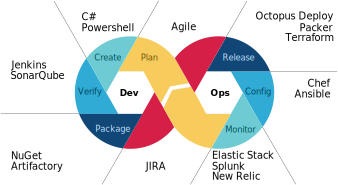
\includegraphics[scale=0.18]{DevOps.pdf}
\vspace{4mm}
}

% Programming skill bars
% DO EDIT THIS FILE DIRECTLY!
% This file is generated from data in YAML file ../../../_data/cv.yaml via 'make cv_update_tex'

\programming{{Bash $\textbullet$ Python $\textbullet$ Golang}, {C $\textbullet$ C++ $\textbullet$ Powershell}, {C\# $\textbullet$ SQL $\textbullet$ Entity Framework}}

\iac{{Powershell DSC  $\textbullet$ Packer}, {Terraform $\textbullet$ Ansible $\textbullet$ Chef}}

\oses{{Mac OS X}, {Windows $\textbullet$ Linux (Ubuntu)}}

\platforms{{Xbox 360 $\textbullet$ PS3 $\textbullet$ iOS $\textbullet$ Android}, {VMware $\textbullet$ Docker $\textbullet$ Kubernetes}, {AWS (EC2, S3, RDS, Lambda, Kinesis)}}

\cicd{{Octopus Deploy $\textbullet$ GitLab}, {Jenkins $\textbullet$ GoCD $\textbullet$ Artifactory}}

\monitoring{{Influxdb $\textbullet$ Grafana}, {Elastic Stack $\textbullet$ Splunk $\textbullet$ New Relic}, {Azure Application Insights}}

\alerting{{Zabbix $\textbullet$ PagerDuty}}


% Projects text
% DO EDIT THIS FILE DIRECTLY!
% This file is generated from data in YAML file ../../../_data/cv.yaml via 'make cv_update_tex'

\projects{
  \textbf{\href{http://johnpaulnewman.com/projects/motor-loan-website/}{Motor Loan Website}}
  \begin{itemize}[noitemsep,topsep=-5pt]
    \item C\# .NET Core
    \begin{itemize}[noitemsep,topsep=-5pt]
      \item AWS SDK for .NET, SignalR
      \item Dapper, Polly
      \item Serilog, Application Insights
      \item Moq, xUnit
    \end{itemize}
    \item Azure
    \begin{itemize}[noitemsep,topsep=-5pt]
      \item Azure Active Directory (AAD) \\Authentication
      \item App Service (Web App)
      \item App Configuration, Key Vault
      \item Event Grid
      \item Log Analytics
    \end{itemize}
    \item AWS
    \begin{itemize}[noitemsep,topsep=-5pt]
      \item AWS RDS MySQL Database
      \item S3 Buckets
      \item SSH Tunnel from Azure to AWS
    \end{itemize}
    \item JQuery with AJAX \\
  \end{itemize}
\textbf{\href{http://johnpaulnewman.com/projects/data-pipeline/}{Data Pipeline}}
\begin{itemize}[noitemsep,topsep=-5pt]
  \item AWS Lambda (C\# \& Python)
  \item AWS Kinesis
  \item AWS Glue \& Athena
  \item AWS EMR (Scala \& PySpark)
  \item Apache Avro \\
\end{itemize}
\textbf{\href{http://johnpaulnewman.com/projects/papers-ocr-solution/}{OCR Solution - Hackathon : Winner}}
\begin{itemize}[noitemsep,topsep=-5pt]
  \item Python (Flask, Celery, RethinkDB)
  \item RabbitMQ \\
\end{itemize}
\textbf{\href{http://johnpaulnewman.com/projects/reporting-service/}{Reporting Service}}
\begin{itemize}[noitemsep,topsep=-5pt]
  \item C\# (Entity Framework, AutoMapper)
  \item JQuery \& d3.js \\
\end{itemize}
\textbf{\href{http://johnpaulnewman.com/projects/gerrit-backup-solution/}{Gerrit Backup Solution}}
\begin{itemize}[noitemsep,topsep=-5pt]
  \item Python \& AWS S3 \\
\end{itemize}
\textbf{\href{http://johnpaulnewman.com/projects/csharp-dependencies-graph/}{C\# Dependencies Graph}}
\begin{itemize}[noitemsep,topsep=-5pt]
  \item Ruby \& JQuery, Graphviz \& SVG \\
\end{itemize}
\textbf{\href{http://johnpaulnewman.com/projects/chef-lwrp/}{Chef LWRP}}
\begin{itemize}[noitemsep,topsep=-5pt]
  \item Chef \& Powershell \\
\end{itemize}
\textbf{\href{http://johnpaulnewman.com/projects/palm-os-rsrc-extractor/}{Palm OS RSRC Extractor}}
\begin{itemize}[noitemsep,topsep=-5pt]
  \item C++, MFC \\
\end{itemize}
\textbf{\href{http://johnpaulnewman.com/projects/adobe-photoshop-automation/}{Adobe Photoshop Automation}}
\begin{itemize}[noitemsep,topsep=-5pt]
  \item C++, COM \\
\end{itemize}
\textbf{\href{http://johnpaulnewman.com/projects/translation-memory-validation/}{Translation Memory Validation}}
\begin{itemize}[noitemsep,topsep=-5pt]
  \item VBScript, Classic ASP, \\XSLT with Javascript functions \\
\end{itemize}
}


% Qualifications
\qualifications{
\textbf{Certificate in C++ Programming}\\\textsc{Open University (MT262 Module)\vspace{1.25mm}} \\
\textbf{Certificate in Programming}\\\textsc{Cambridge Information Technology \\(Pascal \& Delphi)\vspace{1.25mm}} \\
\textbf{BTEC 1st Diploma in Science \& Health} \\
12 Distinctions and 4 Merits
}


%----------------------------------------------------------------------------------------
%   PERSONAL INFORMATION
%----------------------------------------------------------------------------------------
% If you don't need one or more of the below, just remove the content leaving the command, e.g. \cvnumberphone{}

% Info
% DO EDIT THIS FILE DIRECTLY!
% This file is generated from data in YAML file ../../../_data/cv.yaml via 'make cv_update_tex'

% CV Title
\cvname{
  \textbf{JOHN PAUL \vspace{2mm}}\\\textbf{NEWMAN}
}

% Job Title
\cvjobtitle{Senior Software Engineer \vspace{1.0mm}\\ DevOps}


% Contacts
% DO EDIT THIS FILE DIRECTLY!
% This file is generated from data in YAML file ../../../_data/cv.yaml via 'make cv_update_tex'

\cvlinkedin{johnpaulnewman} % LinkedIn
\cvgithub{jpnewman} % GitHub
\cvnumberphone{} % Phone number
\cvsite{johnpaulnewman.com} % Personal website
\cvmail{} % Email address


%----------------------------------------------------------------------------------------

\begin{document}

% Stop hyphenation
\hyphenpenalty=10000
\exhyphenpenalty=10000

 % Print the sidebar
\makeprofile

%----------------------------------------------------------------------------------------
%   Summary
%----------------------------------------------------------------------------------------

\section{Summary}
% DO EDIT THIS FILE DIRECTLY!
% This file is generated from data in YAML file ../../../_data/cv.yaml via 'make cv_update_tex'

\summary{Senior Software Engineer with Windows and Linux DevOps experience working in an Agile environment for FinTech PCI-DSS compliant businesses. \\
Highly competent in Windows and Linux automation, using Chef and Ansible. \\
Experienced in infrastructure automation, using Packer and Terraform, on both Amazon Web Services (AWS) and VMware. Implemented High Availability (HA) and Disaster Recovery (DR) best practices. \\
Designed and managed Continuous Integration (CI)/Continuous Deployment (CD) tools, processes, and pipelines.}


%----------------------------------------------------------------------------------------
%   EXPERIENCE
%----------------------------------------------------------------------------------------

\section{Work Experience}
% DO EDIT THIS FILE DIRECTLY!
% This file is generated from data in YAML file ../../../_data/cv.yaml via 'make cv_update_tex'

\begin{twenty}
\twentyitem[0pt]
  {2019}
  {Present}
  {Senior DevOps Engineer}
  {\href{https://www.ratesetter.com/}{RateSetter}/\href{https://metrobankonline.co.uk}{Metro Bank}}
  {England}
  {Senior DevOps Engineer focused on designing, implementing, monitoring and supporting of Azure infrastructure in across all environments.}
  {\begin{itemize}
    \item Automate the deployment, maintenance, and patching of platform infrastructure for all environments, including Production
    \item Implement and support platform logging infrastructure, including Splunk, Azure Application Insights and alerts
    \item Manage project requirements between all key stakeholders, including IT Ops, InfoSec, Developers, and Business
  \end{itemize}}
  {\begin{itemize}
    \item Introduced HashiCorp Terraform for Azure infrastructure
    \item Created a process for development teams to request infrastructure via Pull Requests (PRs)
    \item Introduced Terraform infrastructure change sign-off and promotion processes using BitBucket PRs and branches
    \item Designed and implemented Azure API Management and Service Bus for a key Metro Bank loan origination platform
    \item Redesigned Azure Service Fabric with Azure best practices
    \item Implemented Azure App Services for both Website and Azure Functions
    \item Developed a C\# ASP.NET Core website to display historical motor loans backed by an AWS RDS MySQL Database and S3 Buckets
  \end{itemize}
  }
\end{twenty}

\vspace{0.25\baselineskip}
\begin{twenty}
\twentyitem
  {2012}
  {2019}
  {Senior Software Engineer/DevOps}
  {Wonga}
  {Ireland - England}
  {Senior Software Engineer within the Platform Engineering Team, focused on DevOps automation, CI/CD, tooling and platform projects like AWS Data Pipeline.}
  {\begin{itemize}
    \item Migration of monolithic application to Service Oriented Architecture (SOA), using NServiceBus MSMQ with DTC.
    \item Implement and maintain Continuous Integration (CI) and Continuous Deployment (CD) systems, including Jenkins, Artifactory, Gerrit, Octopus Deploy
    \item Create Chef and Ansible playbooks for CI/CD servers
    \item Create HashiCorp Terraform for AWS and VMware architecture
    \item Create HashiCorp Packer templates for AWS AMIs and VMware
    \item Implement High Availability (HA) and Disaster Recovery (DR) best practices
    \item Act as interim Scrum Master and Team Leader
  \end{itemize}
  }
  {\begin{itemize}
    \item Introduced the use of NuGet, Artifactory, and Octopus Deploy to manage dependencies and package deployments
    \item Created a process to deploy a legacy VB6 application using Chef, Powershell, and AWS S3
    \item Created a Data pipeline in Python using AWS Lambda, Kinesis, and Glue.
    \item Created Ansible roles to deploy an ELK/Elastic stack, Artifactory, Gerrit, and Jenkins servers
    \item Developed a RESTful Reporting Service using C\#, Entity Framework (EF), JQuery and d3.js
    \item Created Powershell Domain Specific Language (DSL) build and deploy scripts to replace, Ruby Rake and MSBuild scripts
    \item Developed a Ruby application that generated Graphviz DOT files of Microsoft Visual Studio solution dependencies
    \item Developed and maintained multiple in-house tools using Ruby on Rails, C\#, AWS Simple Queue Service (SQS) and Simple Notification Service (SNS)
  \end{itemize}
  }
\end{twenty}

\vspace{0.25\baselineskip}


\newpage
\makeprofiletwo

\section{Work Experience}
% DO EDIT THIS FILE DIRECTLY!
% This file is generated from data in YAML file ../../../_data/cv.yaml via 'make cv_update_tex'

\begin{twenty}
\twentyitem[0pt]
  {2007}
  {2012}
  {Software Internationalization Engineer II}
  {\href{https://www.popcap.com/}{PopCap Games International}}
  {Ireland}
  {Responsible for source code changes to ensure that flagship games, like PopCap's Bejeweled, Plants vs. Zombies, Peggle, and Zuma, worked in multiple languages.}
  {\begin{itemize}
    \item Internationalization and localization of all flagship games, across multiple platforms (PC, iOS, Xbox 360, PlayStation, Nintendo DS) using multiple development languages including, C++, Objective-C, Flash ActionScript
    \item Liaised with US and APAC project teams to achieve timely delivery of project goals
    \item Acted as point of contact and subject matter expert for Internationalization
  \end{itemize}
  }
  {\begin{itemize}
    \item Reduced art resource requirements by automating Adobe Photoshop to create Asian language Bitmap Fonts
    \item Created a script to import/export text from Photoshop files, allowing for faster translation of graphical assets
    \item Developed numerous Python, JavaScript, and VBA tools to reduce engineering time and resources
    \item Managed multiple key projects simultaneously - liaising with multiple project stakeholders in the US and APAC
    \item Consistently took the initiative to scope new technology requirements and analyse project impacts
  \end{itemize}
  }
\end{twenty}

\vspace{0.25\baselineskip}
\begin{twenty}
\twentyitem
  {2002}
  {2007}
  {Software Internationalization and Build Engineer}
  {\href{https://www.welocalize.com/}{Welocalize/Connect Global Solutions}}
  {Ireland}
  {Lead Engineer on various projects and managing a small team.}
  {}
  {\begin{itemize}
    \item Received client recognition for designing, developing, and implementing an online system in Classic ASP that validated Translation Memories (TMs) and ensured higher leverage
    \item Created extensive GNU Make and Microsoft NMake makefiles for building and deploying applications into multiple locales
    \item Developed C++ tool to extract text from the Palm OS RSRC file format, enabling shorter localization cycles
  \end{itemize}
  }
\end{twenty}

\vspace{0.25\baselineskip}
\begin{twenty}
\twentyitem
  {2000}
  {2002}
  {Software Localization Engineer}
  {\href{https://www.lionbridge.com/}{Bowne Global Solutions}}
  {Ireland}
  {}
  {}
  {\begin{itemize}
    \item Developed numerous Microsoft Word VBA macros to enhance the localization workflow
    \item Developed comprehensive functional test scripts for cutting edge mobile devices, like Handspring VisorPhone
  \end{itemize}
  }
\end{twenty}

\vspace{0.25\baselineskip}
\begin{twenty}
\twentyitem
  {1998}
  {2000}
  {Software Localization Engineer and IT Network Administrator}
  {Tek Translation}
  {England - Ireland}
  {}
  {}
  {\begin{itemize}
    \item Migrated Novell to Windows NT 4 and Pegasus Mail to Exchange Server
    \item Set-up and maintained Sage Line 100, a MS-DOS based accounting system
  \end{itemize}
  }
\end{twenty}

\vspace{0.25\baselineskip}


\end{document}
